\newcommand{\figdistribvpic}{
  \centering
  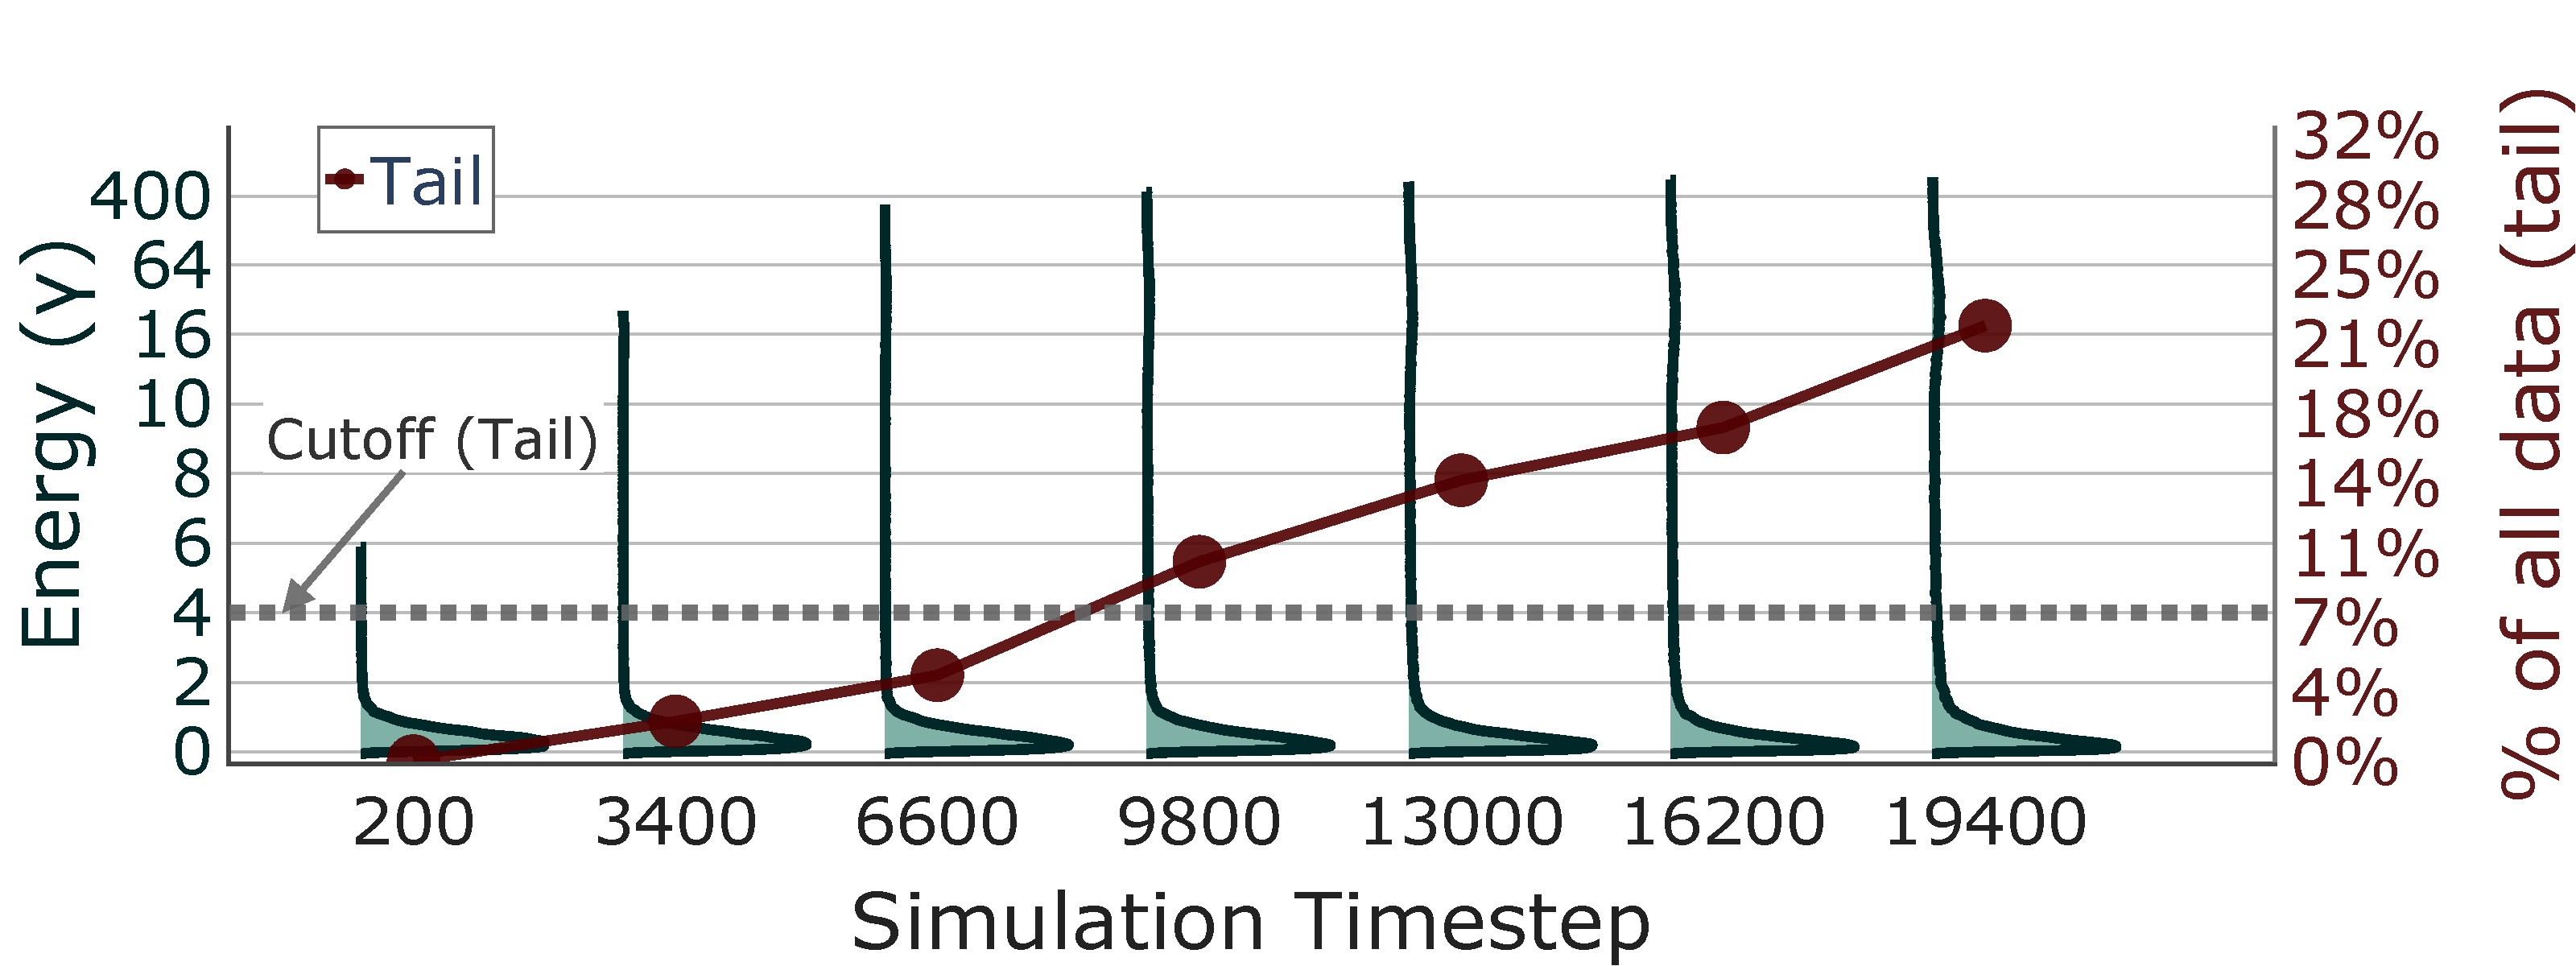
\includegraphics[trim=0cm 0cm 0cm 1.6cm,clip,width=\columnwidth]{data/figs/carp_distrib.vpic.pdf}
  \caption{VPIC Energy Distribution}
  \label{fig:carp:distrib-vpic}
}

\newcommand{\figdistribamr}{
  \centering
  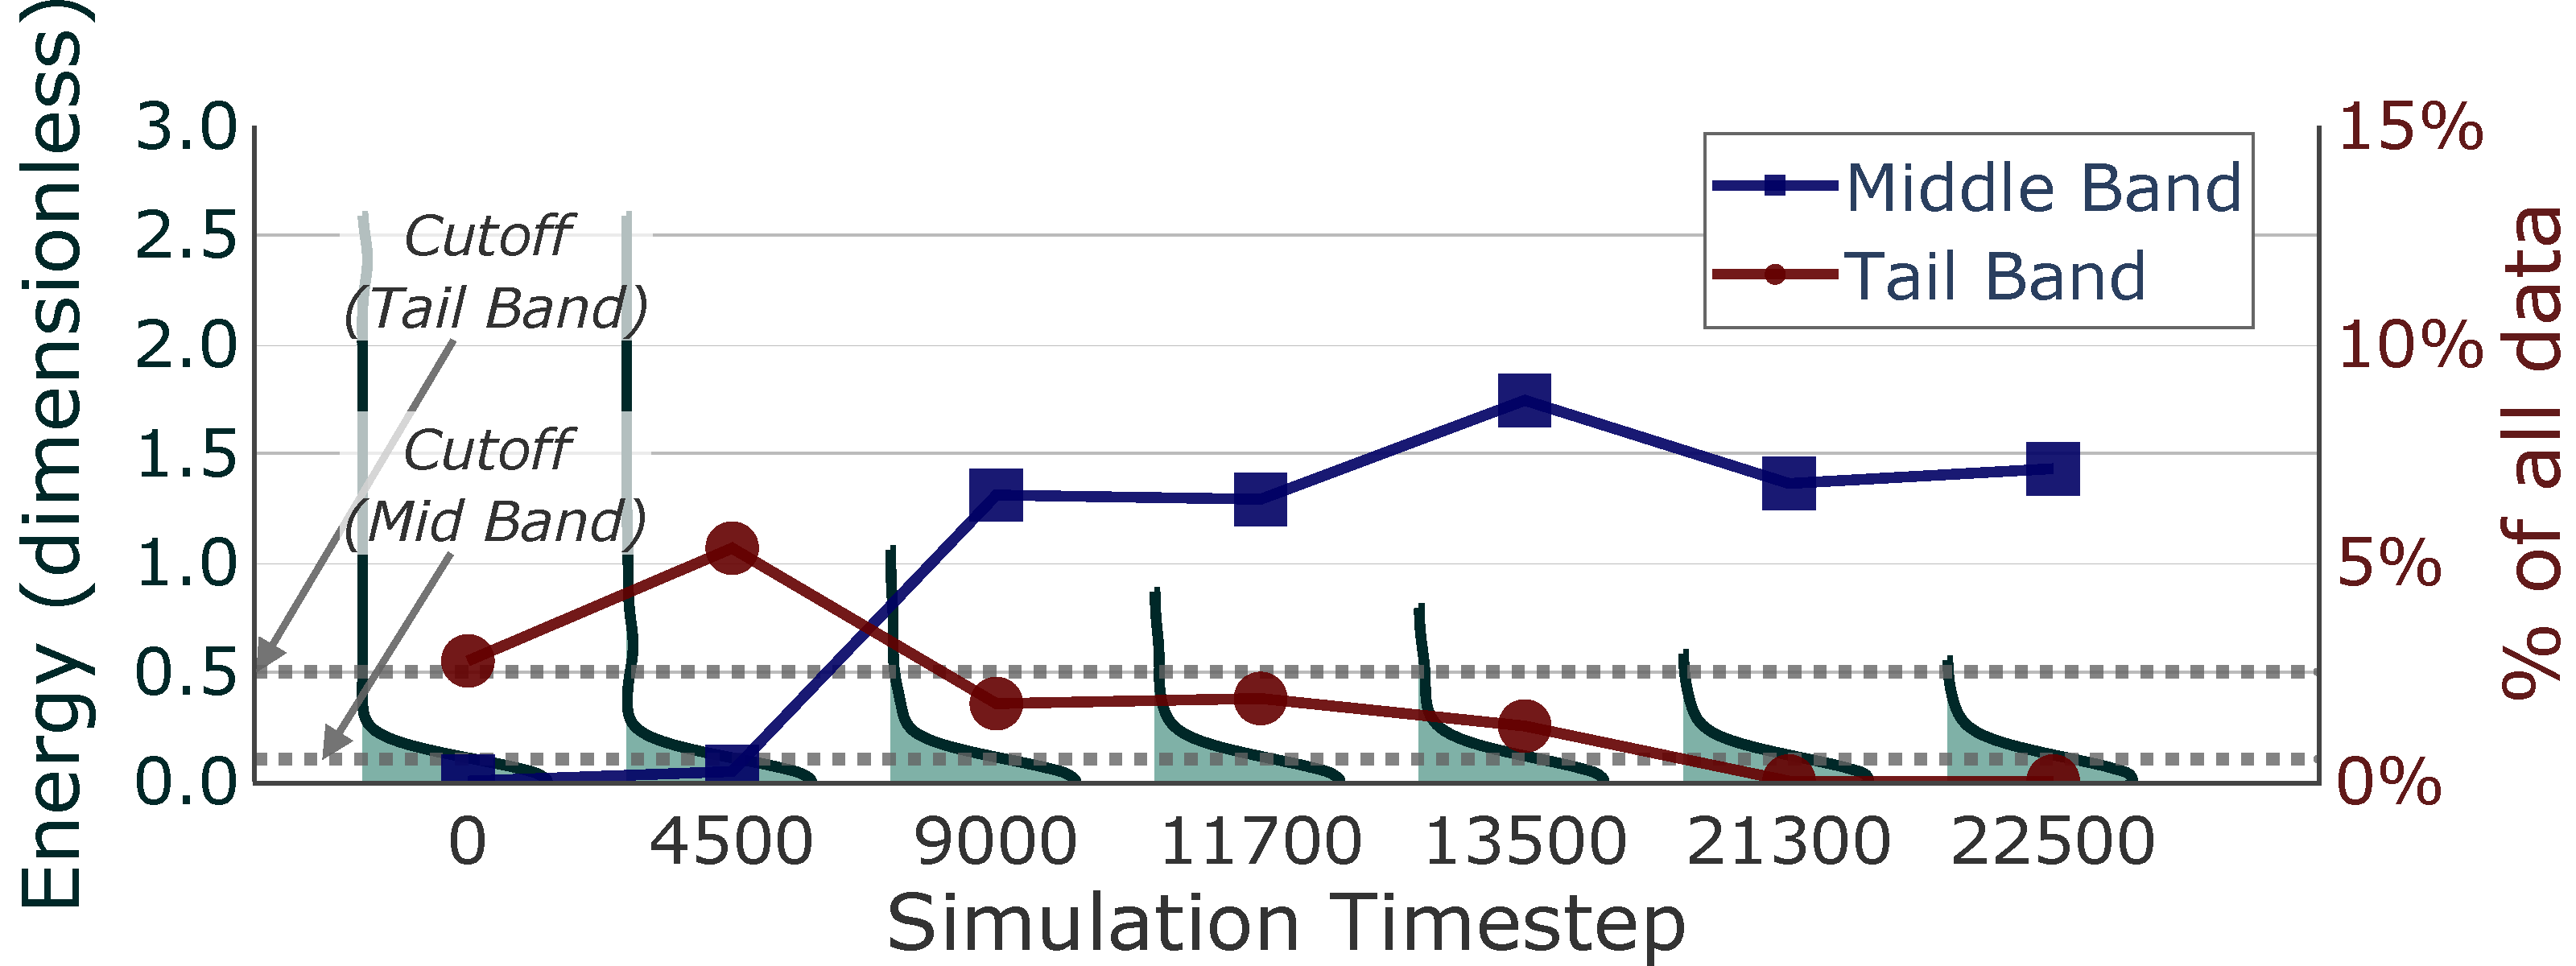
\includegraphics[trim=0cm 0cm 0cm 0cm,clip,width=\columnwidth]{data/figs/carp_distrib.amr.pdf}
  \caption{Adaptive Mesh Refinement Energy Distribution}
  \label{fig:carp:distrib-amr}
}

\newcommand{\capfigdistrib} {
  \caption{Energy distributions across 7 timesteps of VPIC (top) and AMR (bottom) simulations.
    Distributions are shows as histograms overlaid with line plots for interesting bands.
Both VPIC and AMR distributions are highly skewed and shift significantly over time.
  }
  \label{fig:carp:distrib}
}

\newcommand{\figdeslayout}{
  \centering
  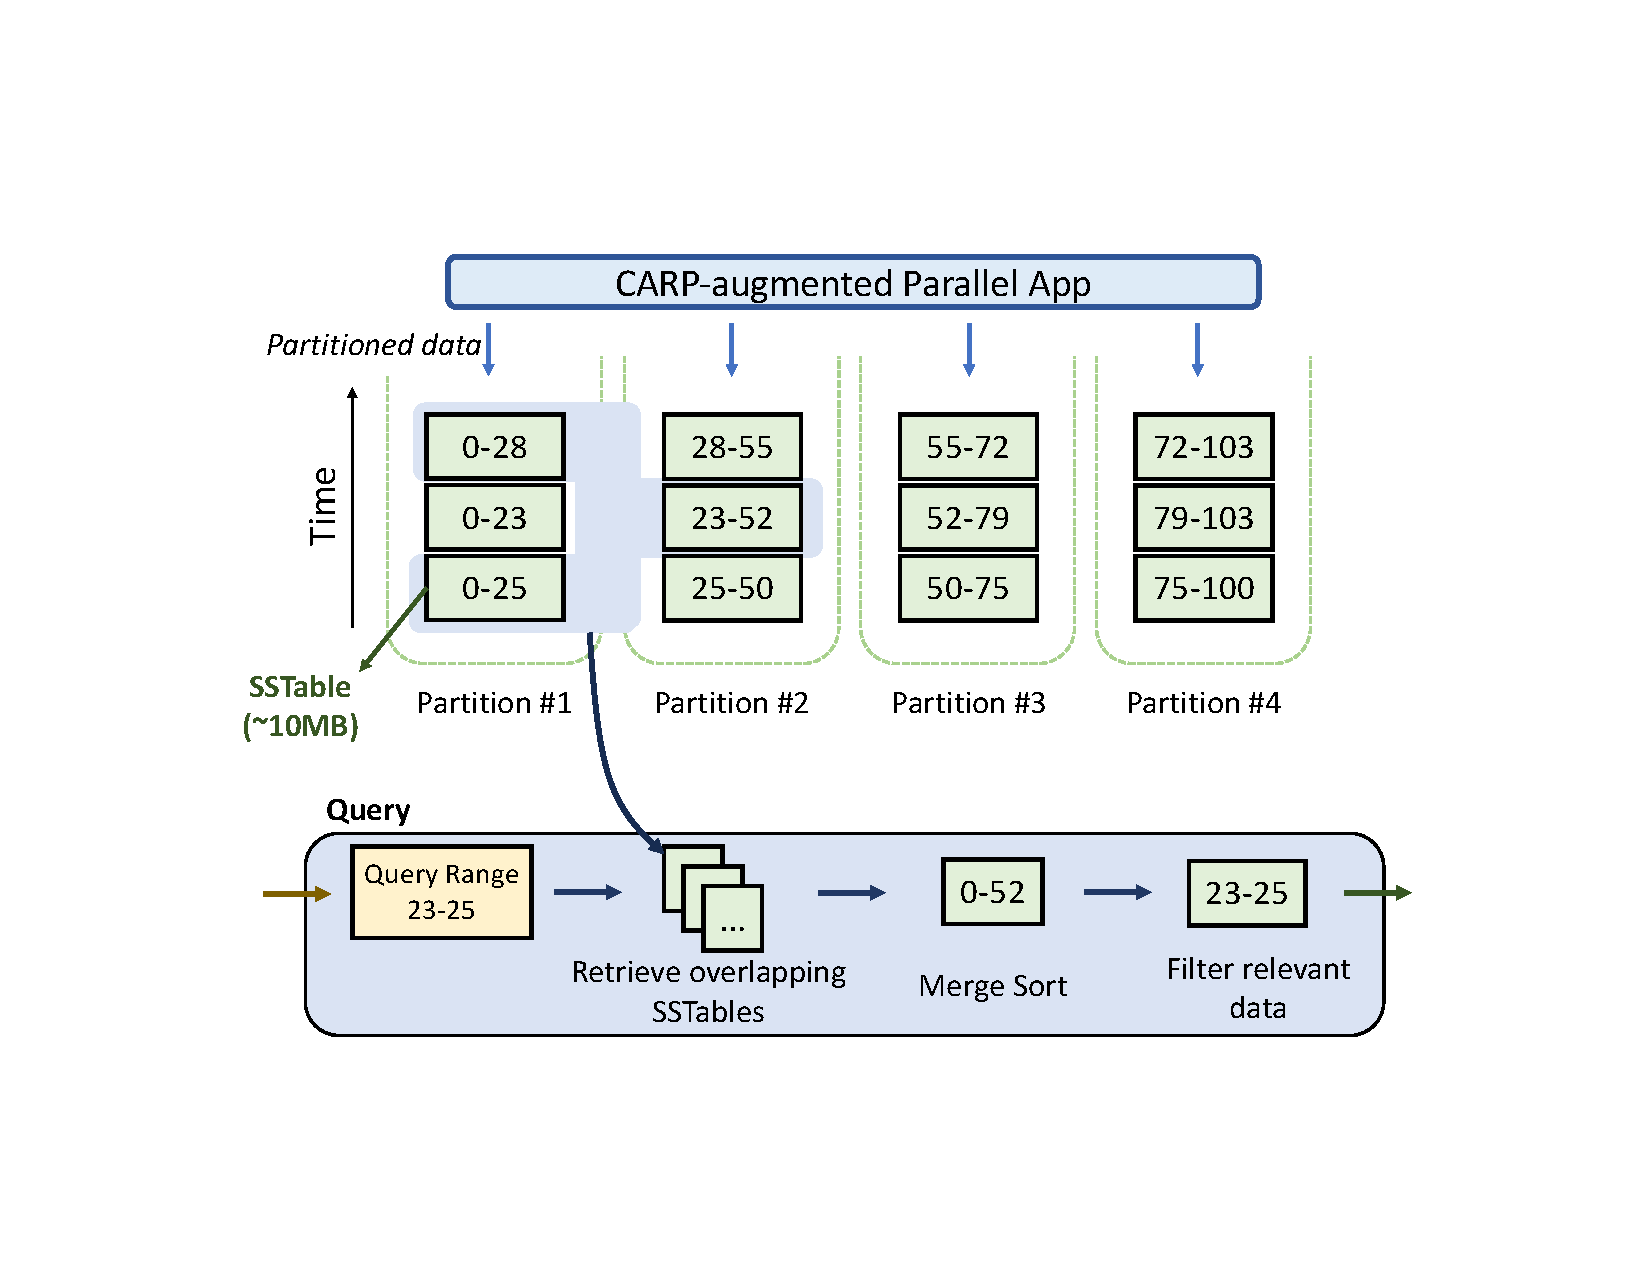
\includegraphics[trim=3.5cm 4.0cm 3.5cm 4.3cm,clip,width=\columnwidth]{data/figs/carp_layout_v2.pdf}
  \caption{A logical view of CARP's data layout and querying. Incoming data is partitioned and stored as SSTables, and partition boundaries shift with key distribution changes. Queries retrieve relevant SSTables and merge them.}
  \label{fig:carp:des-layout}
}

\newcommand{\figdesarch}{
  \centering
  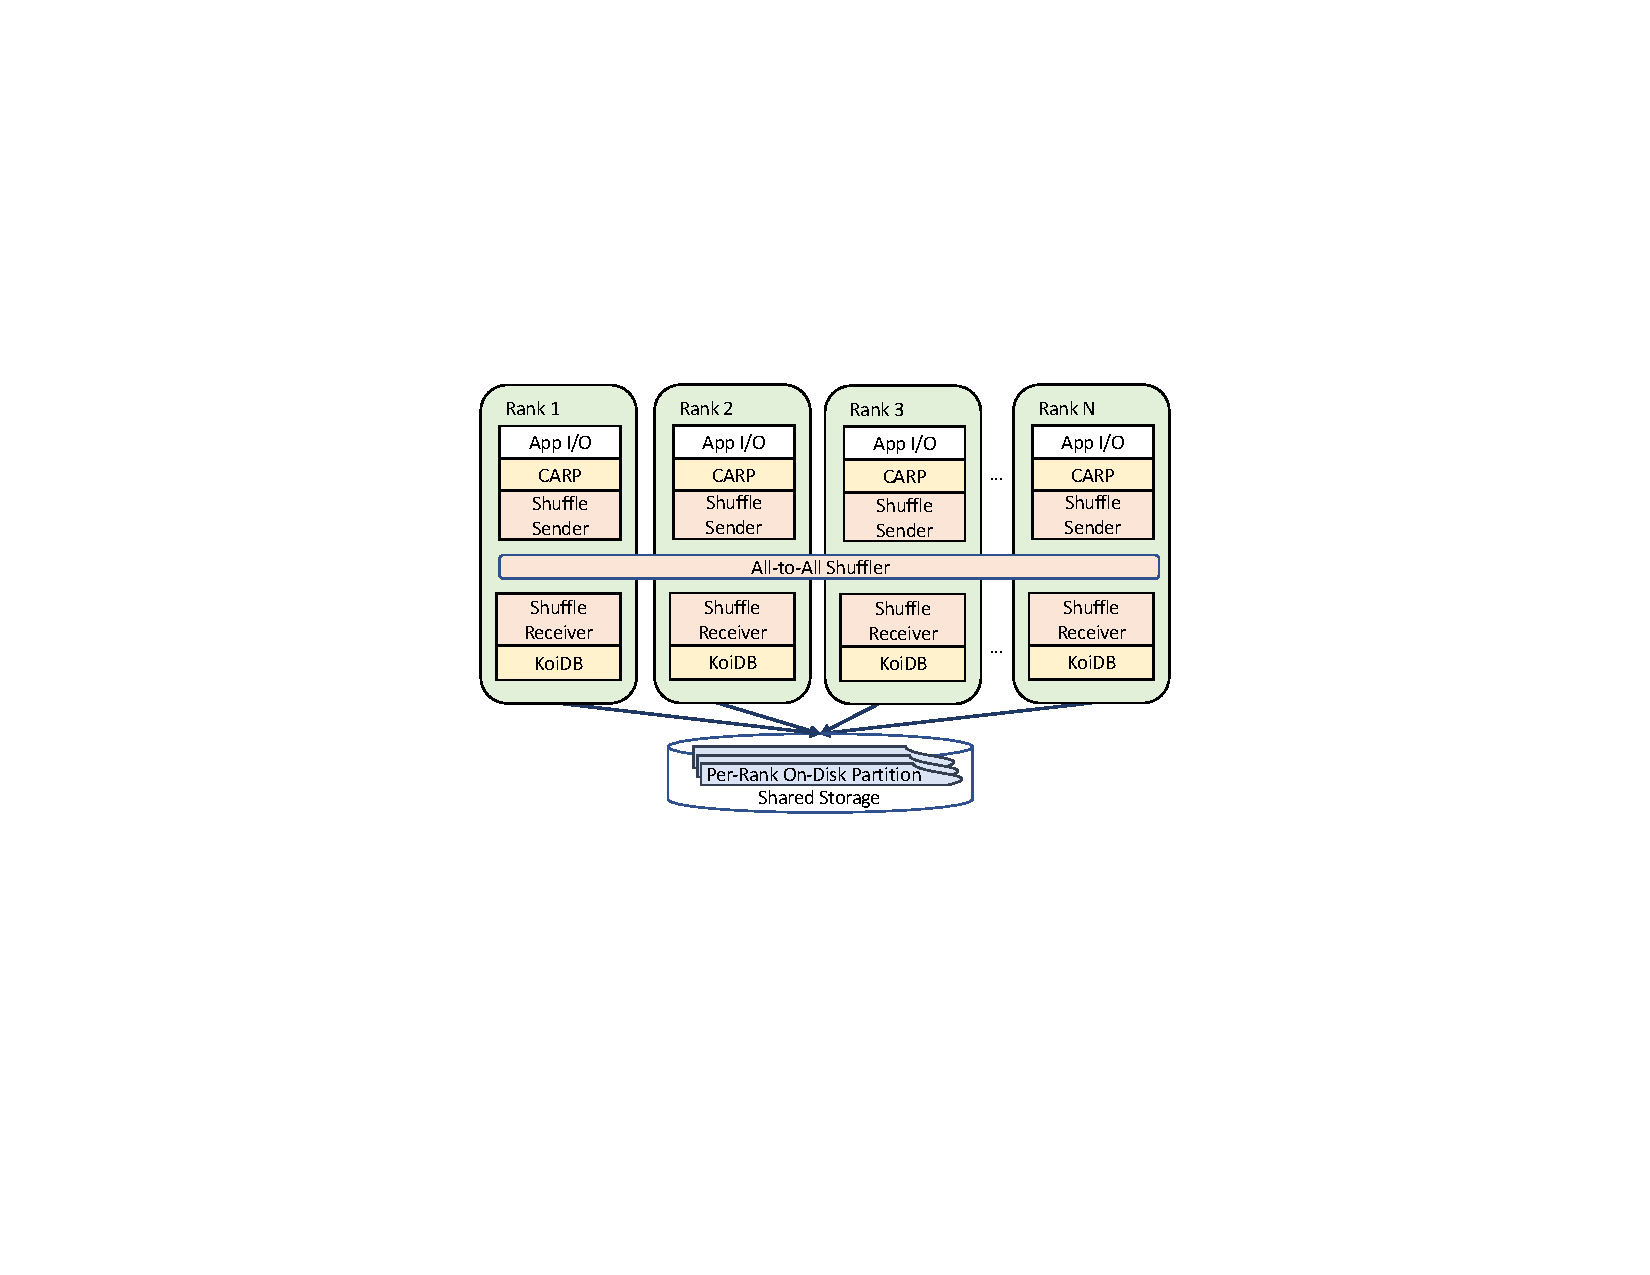
\includegraphics[trim=8cm 7.8cm 8cm 6.5cm,clip,width=0.9\columnwidth]{data/figs/carp_arch_v12mini.pdf}
  \caption{Example of an N-rank application using CARP. Writes are intercepted and partitioned via an all-to-all shuffler. Each rank is both a sender and receiver. Partitioned data collected by receivers is stored by a local storage backend (KoiDB).}
  \label{fig:carp:des-arch}
}

\newcommand{\figdessend}{
  \centering
  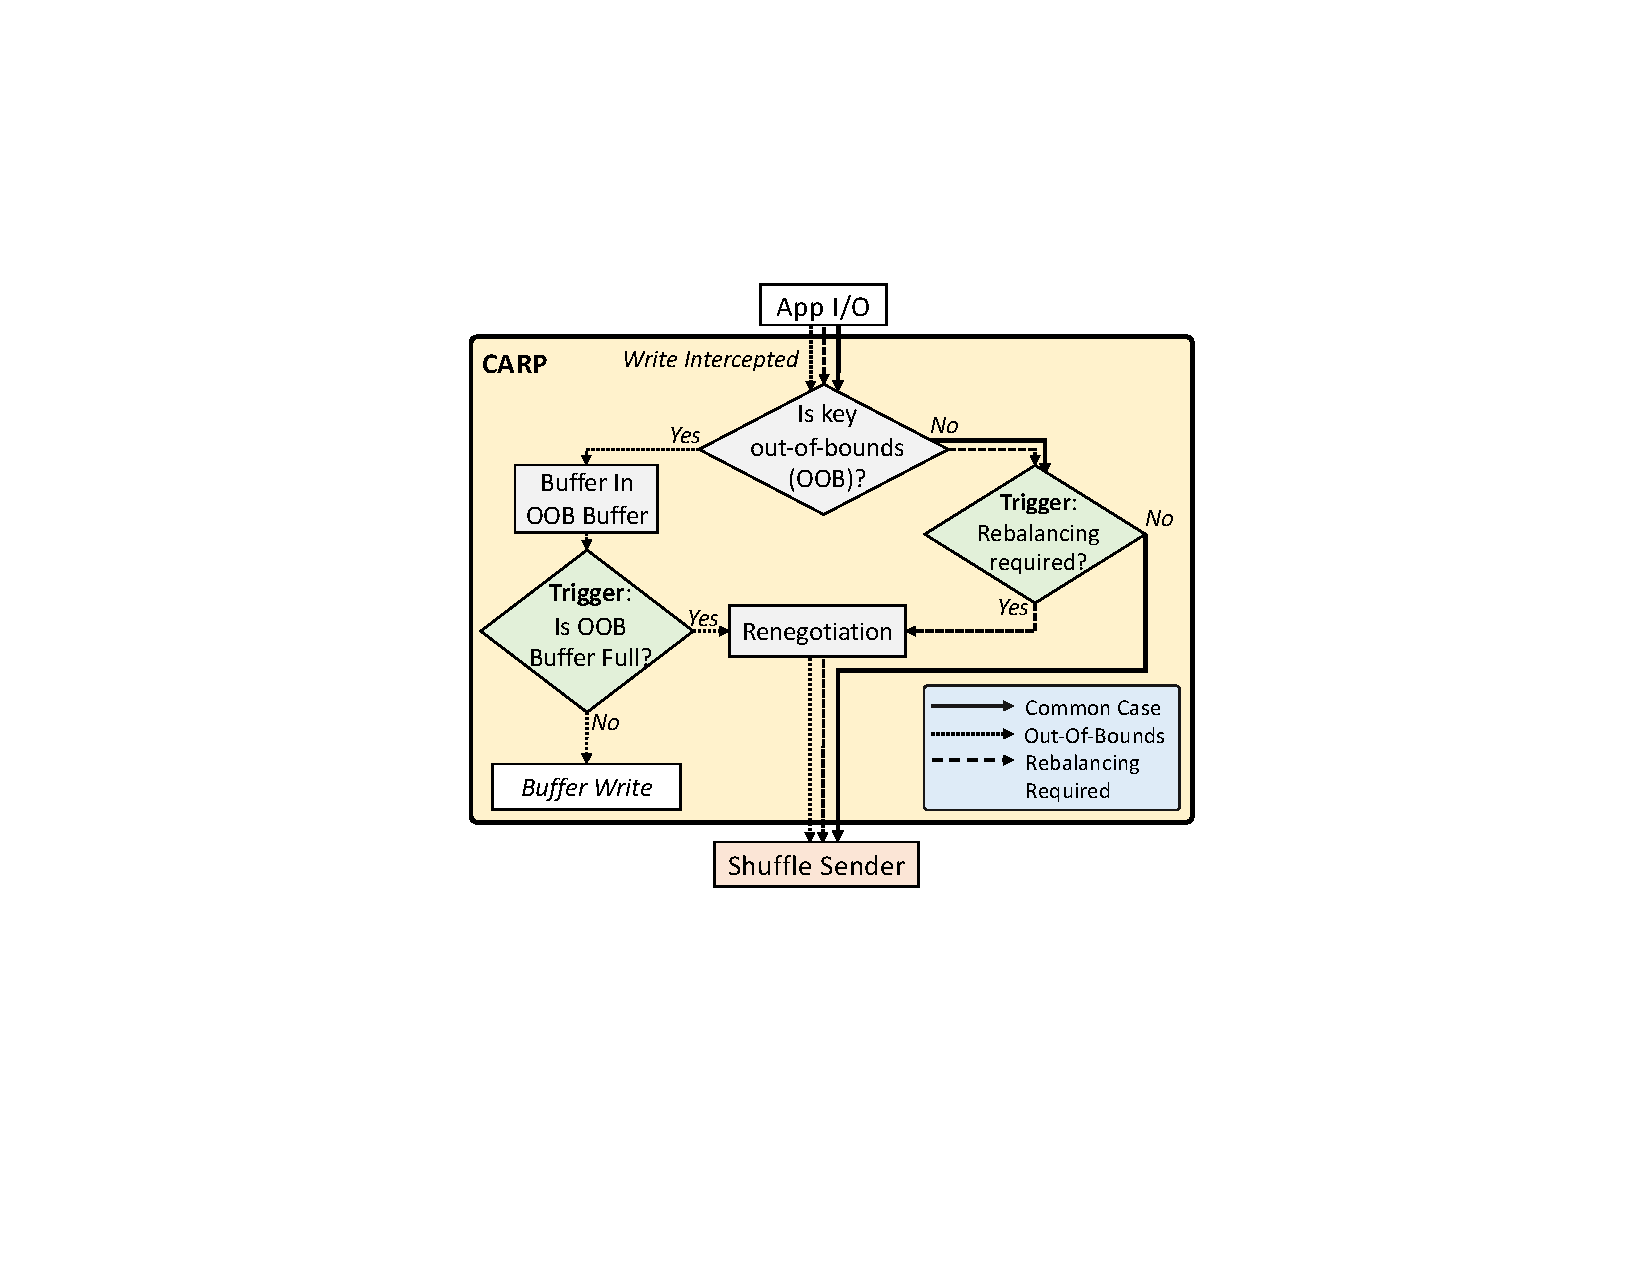
\includegraphics[trim=7.9cm 6.5cm 7.7cm 4.8cm,clip,width=0.85\columnwidth]{data/figs/carp_sender_wobg_v6.pdf}
  \caption{CARP data and control flow. Application data is routed by the shuffle sender to its partition. But, if its key is outside all partition bounds, then data is added to an Out-Of-Bounds (OOB) buffer. When the OOB buffer fills up or partitions become imbalanced, CARP renegotiates the partition table.}
  \label{fig:carp:des-send}
}

\newcommand{\figdeshist}{
  \centering
  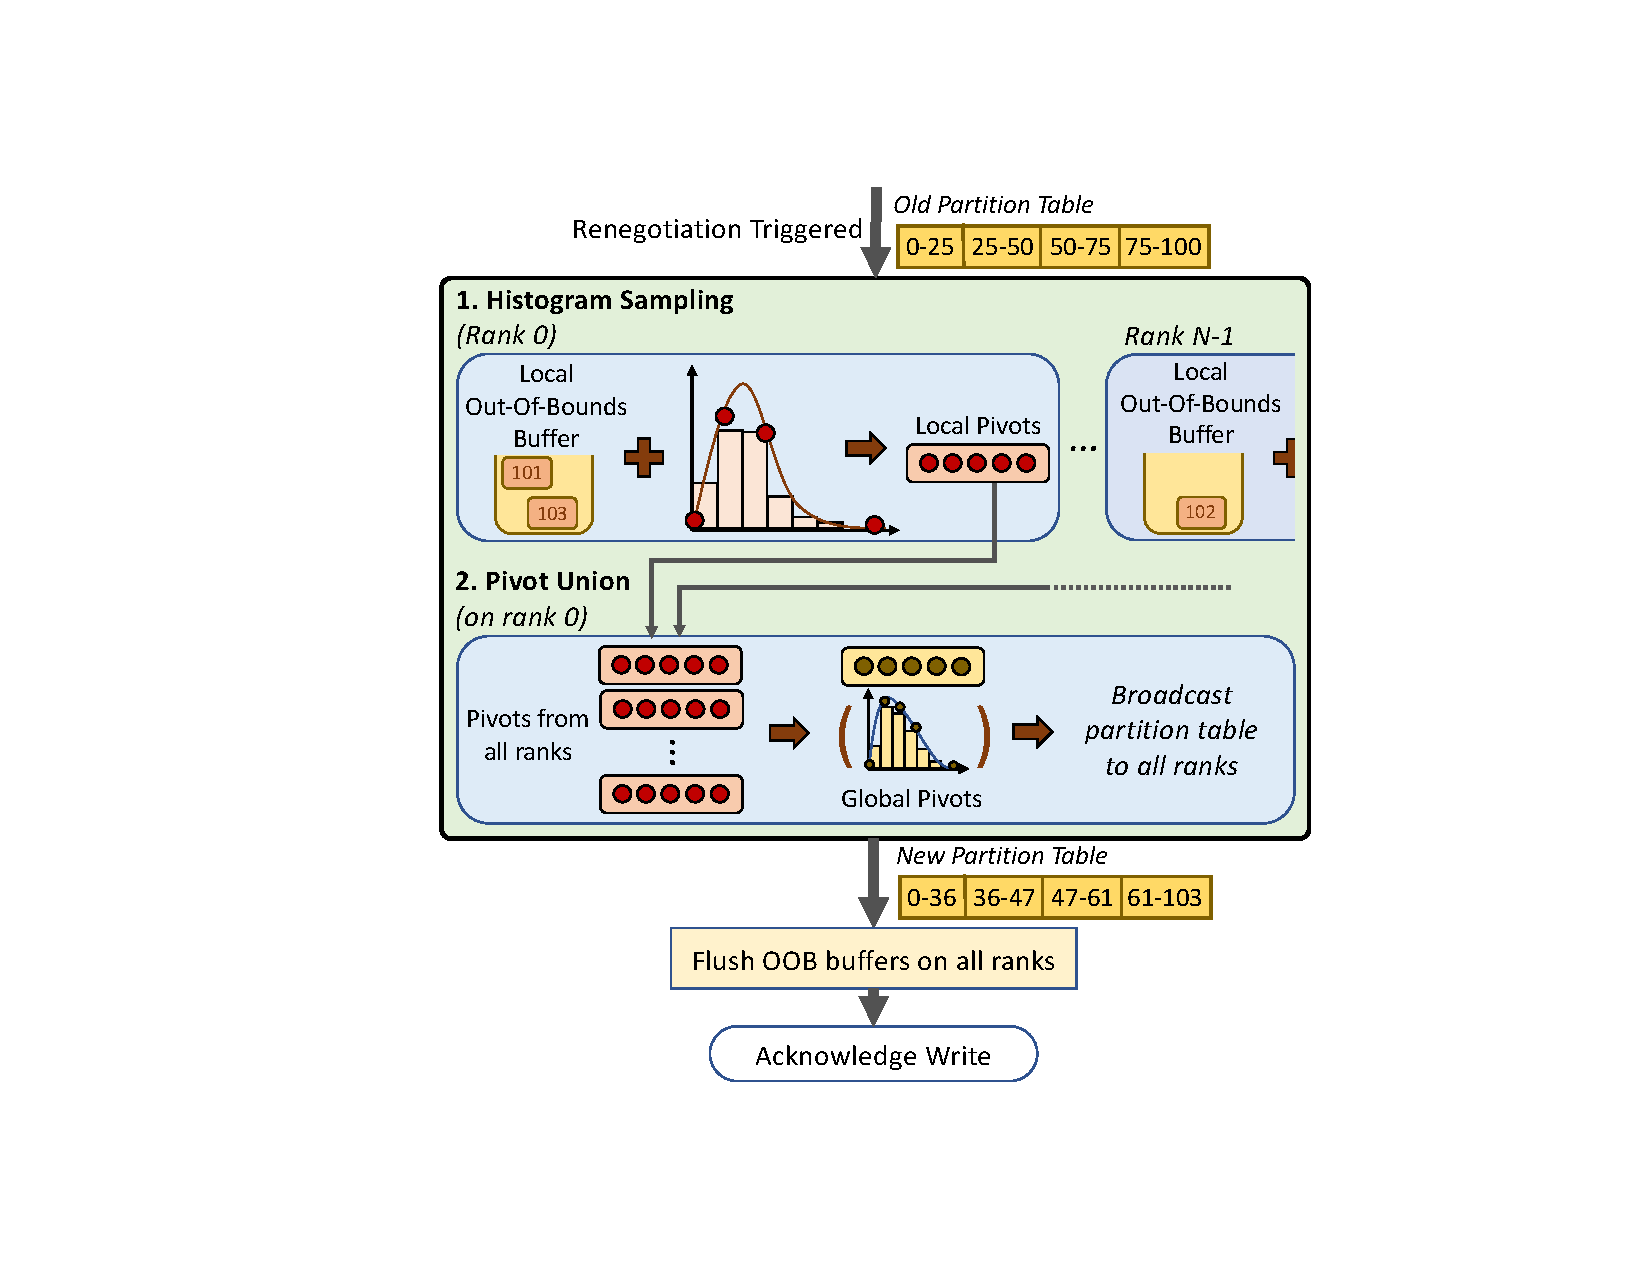
\includegraphics[trim=7.4cm 3.2cm 5.7cm 3.3cm,clip,width=0.9\columnwidth]{data/figs/carp_reneg_hists_v4.pdf}
  \caption{Partition table renegotiation relies on pivots computed from histograms of keys tracked on each rank. Pivots are merged, and the new global histogram is divided into equal-mass bins before being broadcasted.
  }
  \label{fig:carp:des-hist}
}

\newcommand{\figdeskoidb}{
  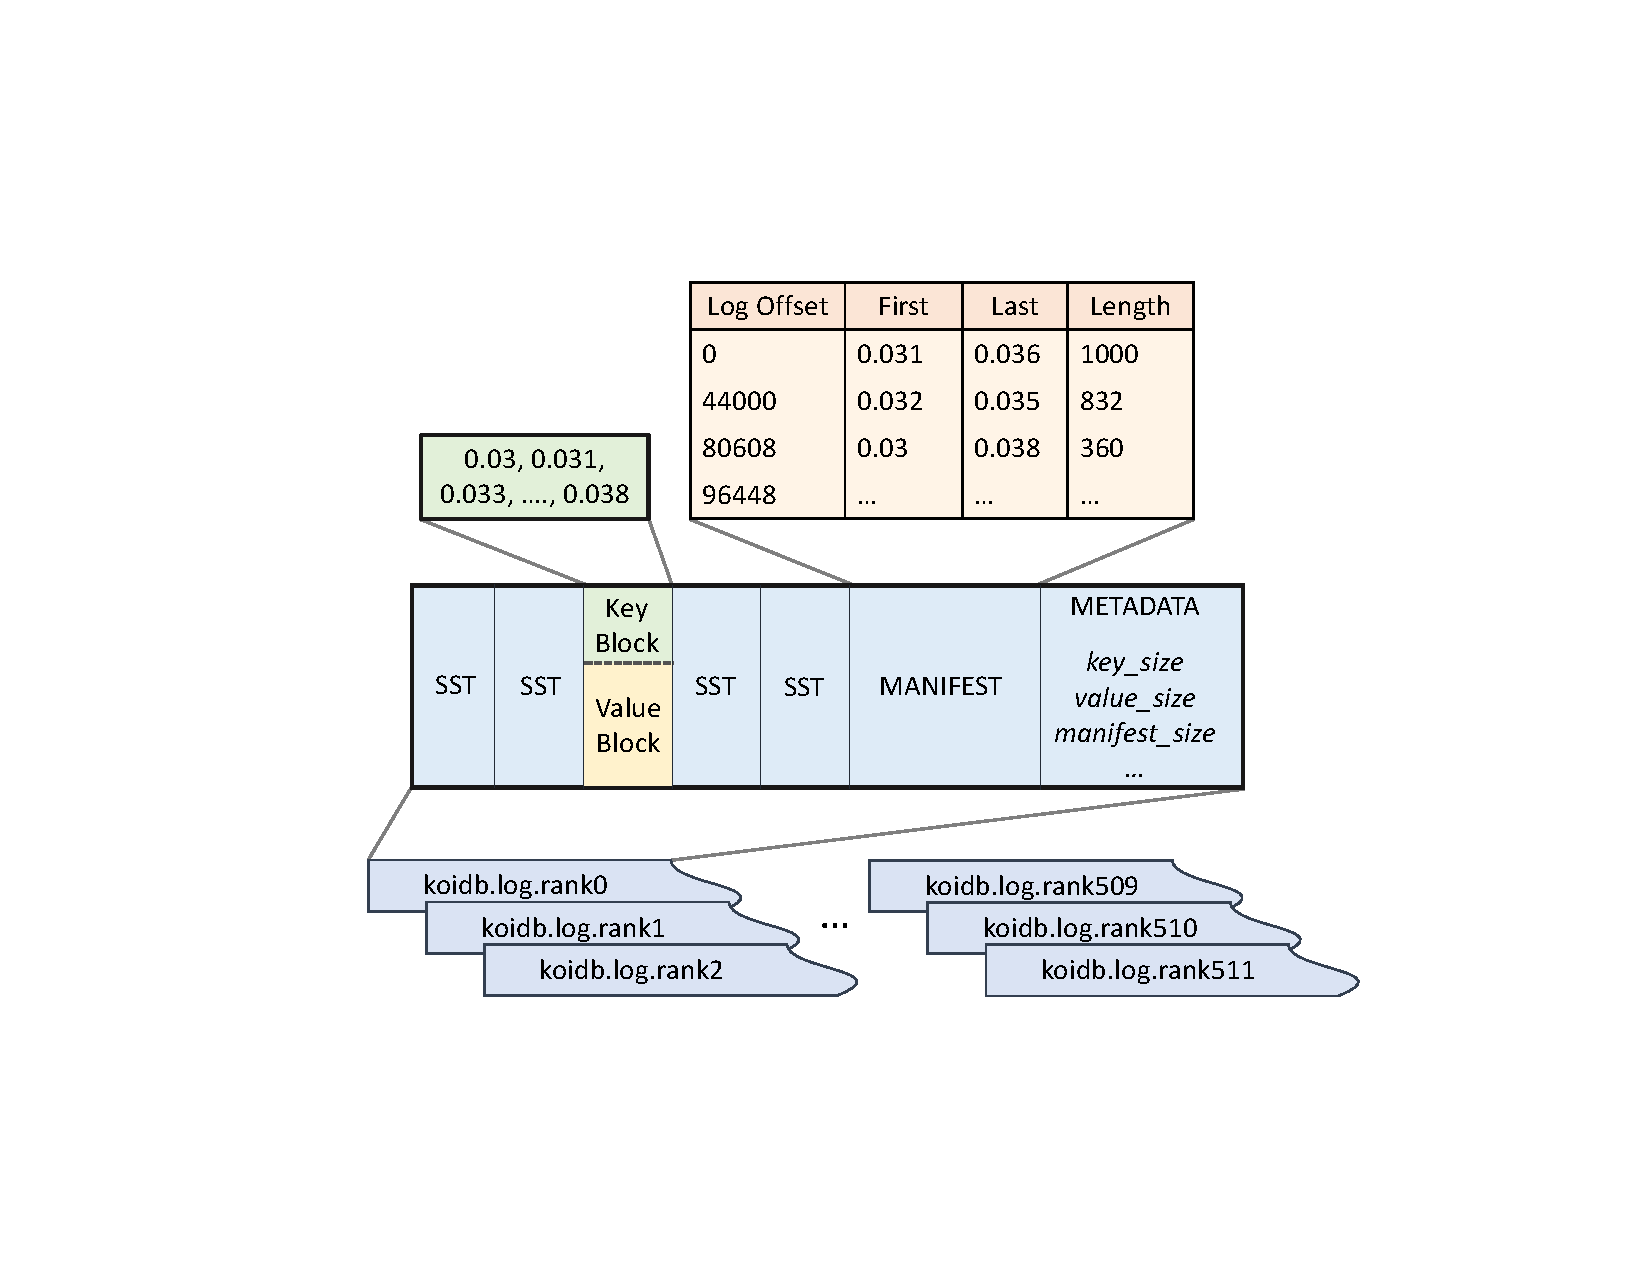
\includegraphics[trim=6cm 4cm 4cm 4.7cm,clip,width=0.5\textwidth]{data/figs/carp_carpdb_log_v3.pdf}
  \caption{KoiDB on-disk log format. Each log consists of SSTables organized into contiguous key and value blocks. Each SST has an entry in the manifest along with metadata.
  }
  \label{fig:carp:des-carpdb}
}

\newcommand{\figktqlat} {
  \centering
  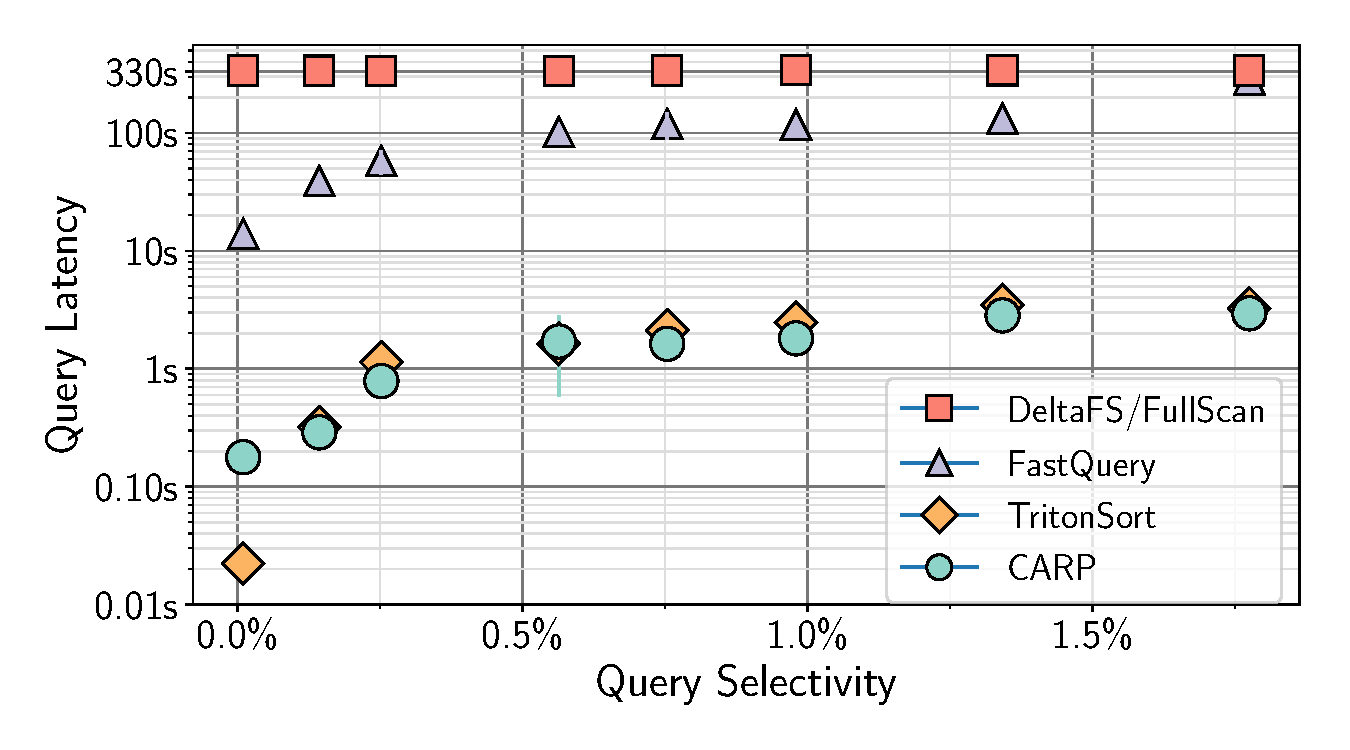
\includegraphics[trim=0.7cm 0.84cm 0.5cm 0.70cm,clip,width=\textwidth]{data/figs/carp_qlatvssel.v6.pdf}
  \caption{Query Latency}
  \label{fig:carp:kt-qlat}
}

\newcommand{\figktrt}{
  \centering
  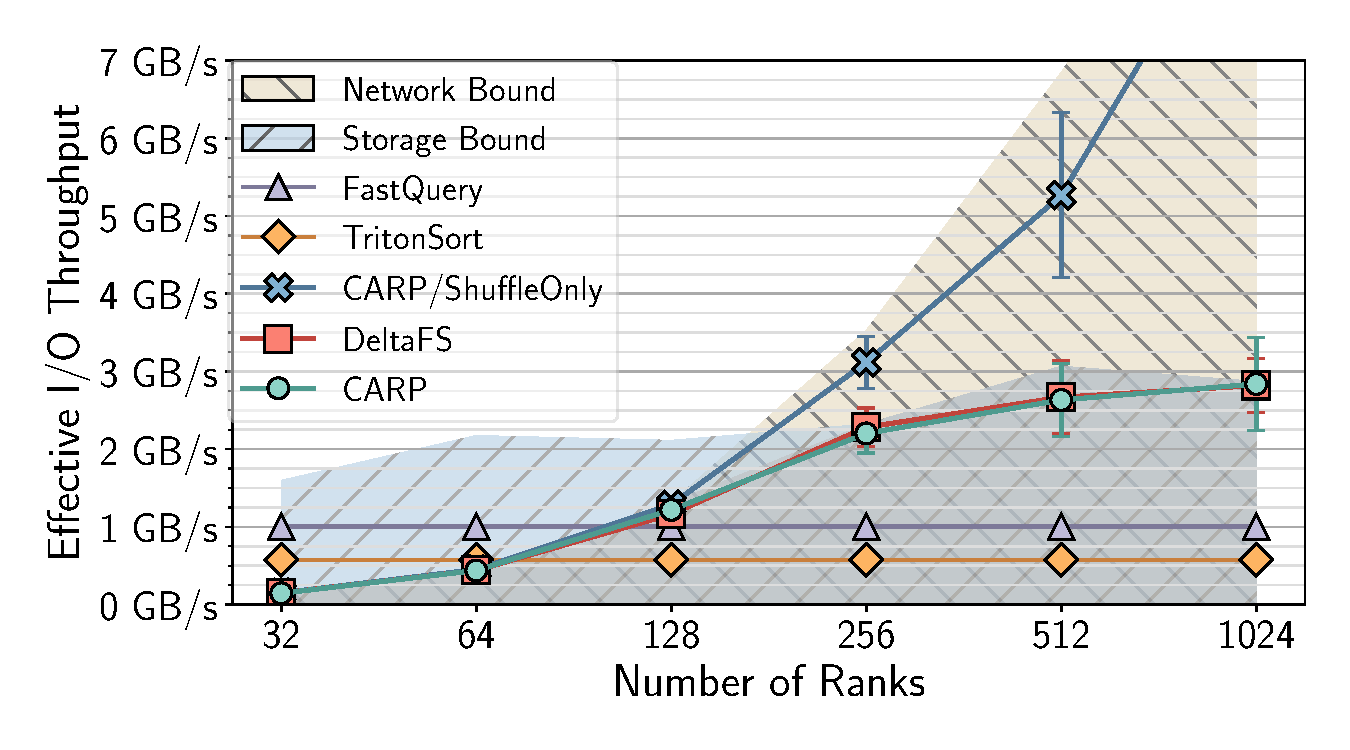
\includegraphics[trim=0.6cm 0.90cm 0.6cm 0.80cm,clip,width=\linewidth]{data/figs/carp_runtime.v4.werr.pdf}
  \caption{I/O Throughput}
  \label{fig:carp:kt-rt}
}

\newcommand{\capfigkt} {
  \caption{(Left) CARP matches the query latency of TritonSort's fully-sorted data layout and outperforms both FastQuery by 100$\times$. (Right) CARP incurs no overhead over unpartitioned I/O and is 3-5$\times$ faster than post-processing.}
}

\newcommand{\figevalycsb}{
  \centering
  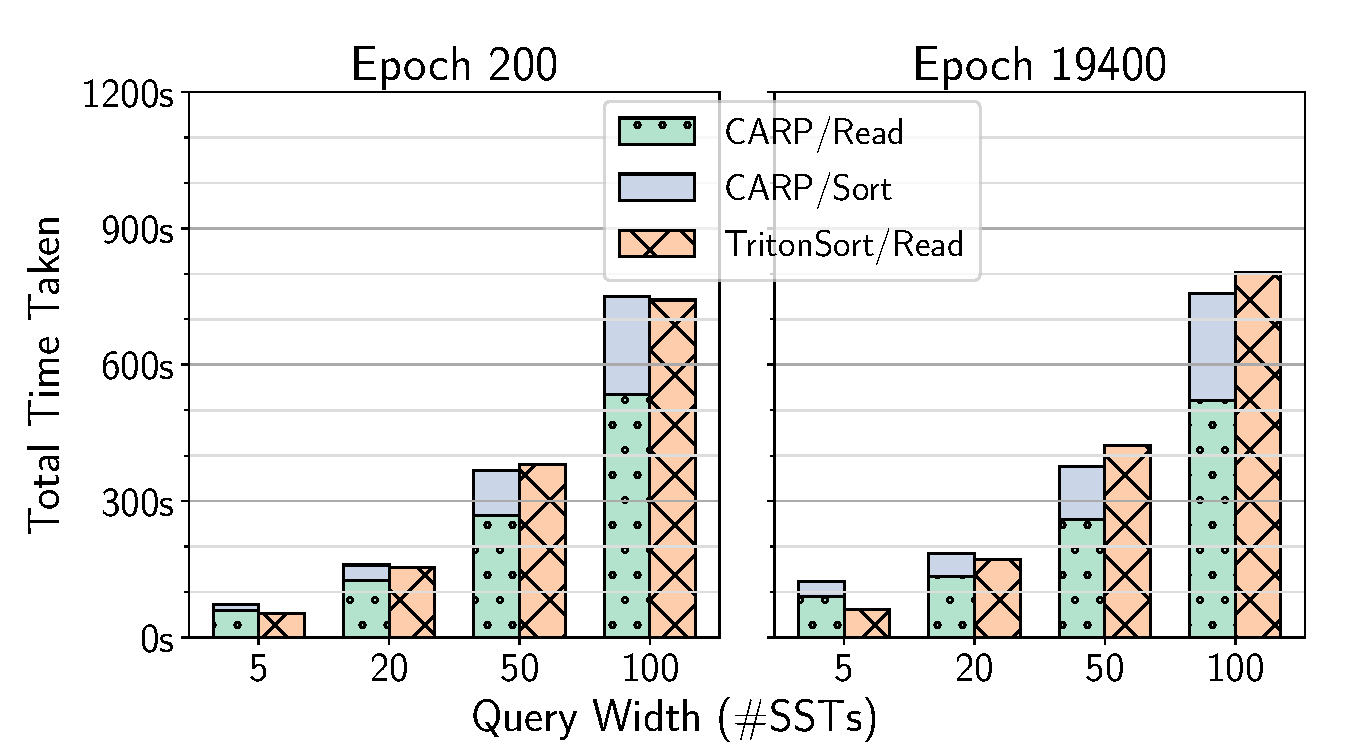
\includegraphics[trim=0.5cm 0.2cm 0.7cm 0.7cm,clip,width=0.9\columnwidth]{data/figs/carp_query.ycsb.v3.pdf}
  \caption{Time taken for a YCSB query suite, demonstrating similar trends to the left-hand figure. CARP is slower for highly selective queries but comparable/better for larger queries despite the sorting overhead.}
  \label{fig:carp:eval-ycsb}
}

\newcommand{\figevaldyn}{
  \centering
  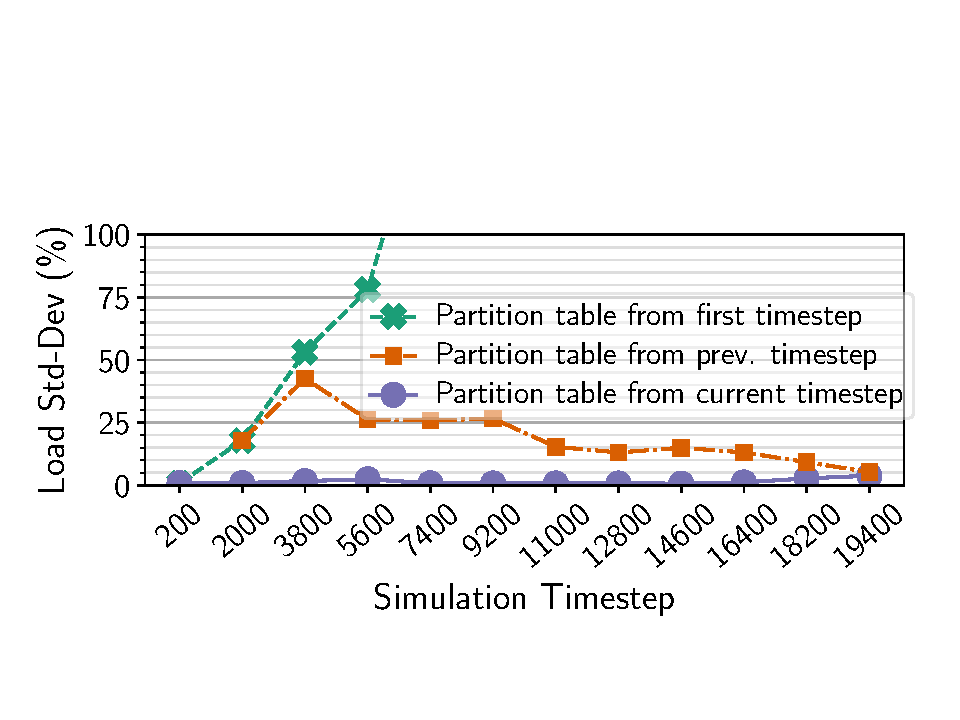
\includegraphics[trim=0.6cm 1.7cm 0.9cm 3.8cm,clip,width=0.9\columnwidth]{data/figs/carp_pvtbench.adapt.pdf}
  \caption{
  Simulated performance of different static partitioning schemes in generating balanced partitions (lower load std-dev implies better partition balance). Reusing a partition table from the first timestep results in the worst load-balance. Tables from the previous timestep fare better, but perform poorly when the simulation is the most active. Tables from the current timestep fit the best (true by definition).
  }
  \label{fig:carp:eval-dyn}
}

\newcommand{\figevalrtplat}{
  \centering
  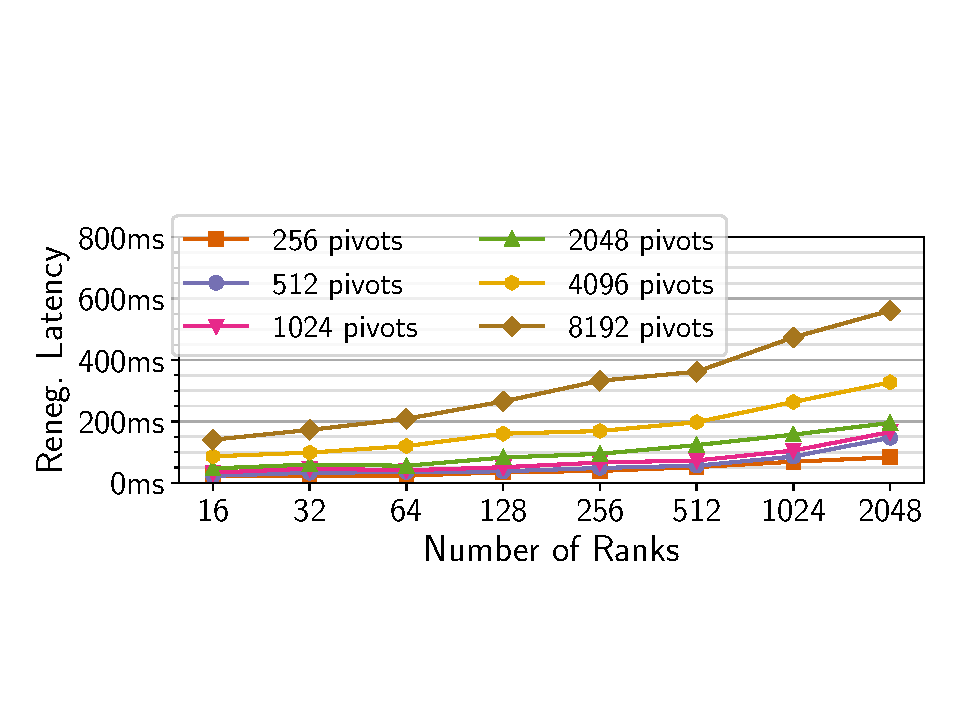
\includegraphics[trim=0.6cm 2.6cm 0.6cm 3.6cm,clip,width=\columnwidth]{data/figs/carp_rtp.latvspvtcnt.pdf}
  \caption{Renegotiation scalability at different pivot counts}
  \label{fig:carp:eval-rtplat}
}

\newcommand{\figevalpvtcnt}{
  \centering
  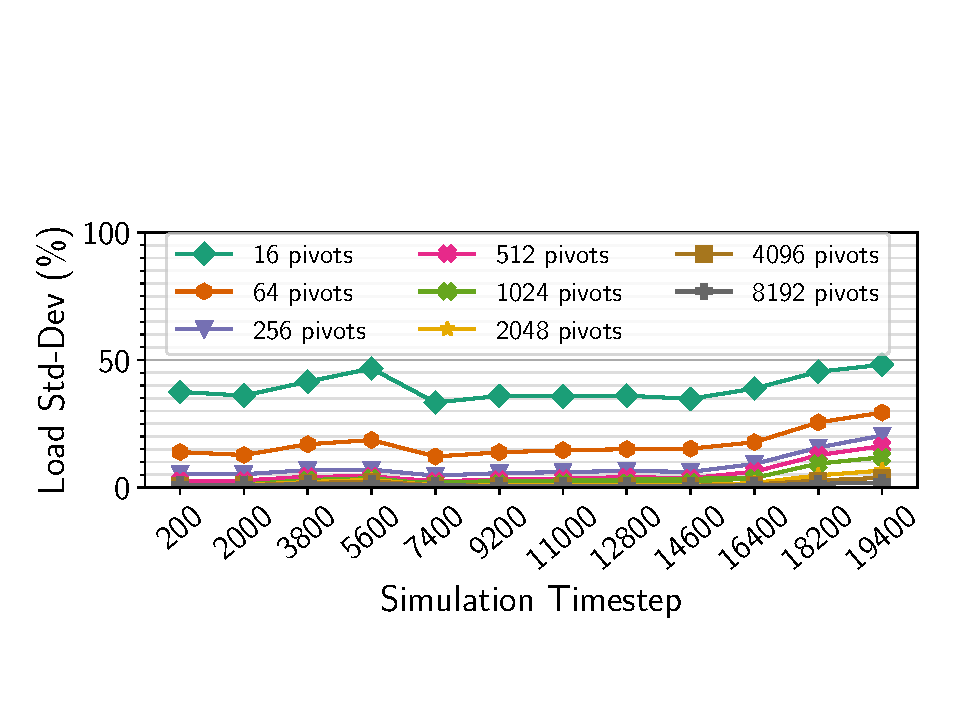
\includegraphics[trim=0.6cm 1.7cm 0.7cm 3.7cm,clip,width=\columnwidth]{data/figs/carp_pvtbench.epxpp.pdf}
  \caption{Pivot Count vs Histogram Fidelity}
  \label{fig:carp:eval-pvtcnt}
}

\newcommand{\figevalcarpdb}{
  \centering
  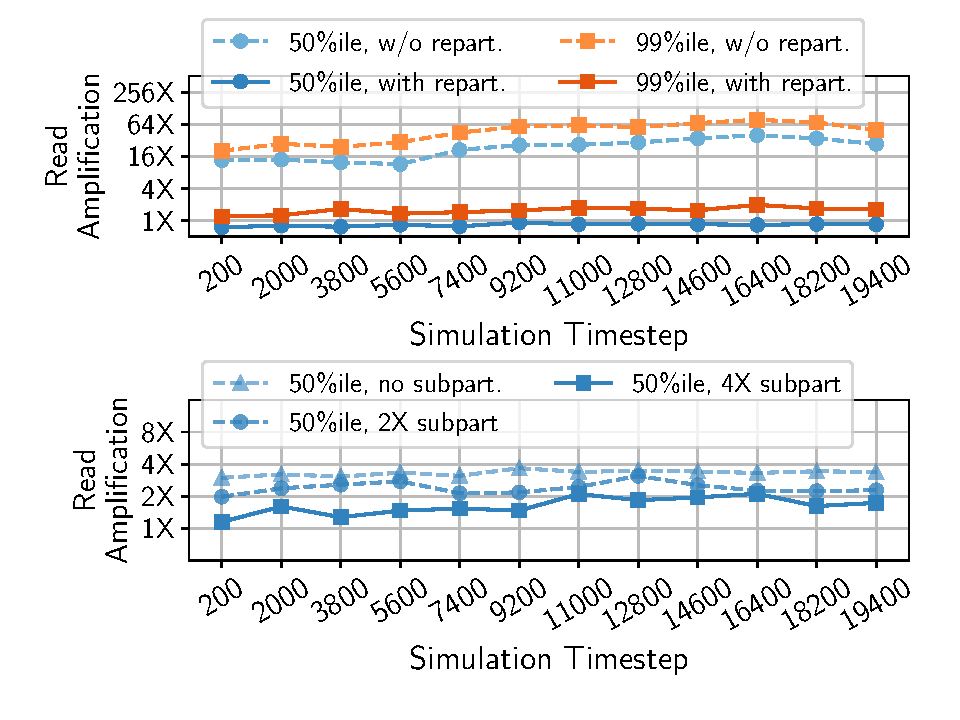
\includegraphics[trim=0.4cm 6.1cm 0.3cm 0cm,clip,width=\columnwidth]{data/figs/carp_carpdb.impact.alt4.pdf}
  \caption{Impact of repartitioning on 50\textsuperscript{th} and 99\textsuperscript{th} percentile RAF}
  \label{fig:carp:eval-carpdb}
}

\newcommand{\figevalrtpload}{
  \centering
  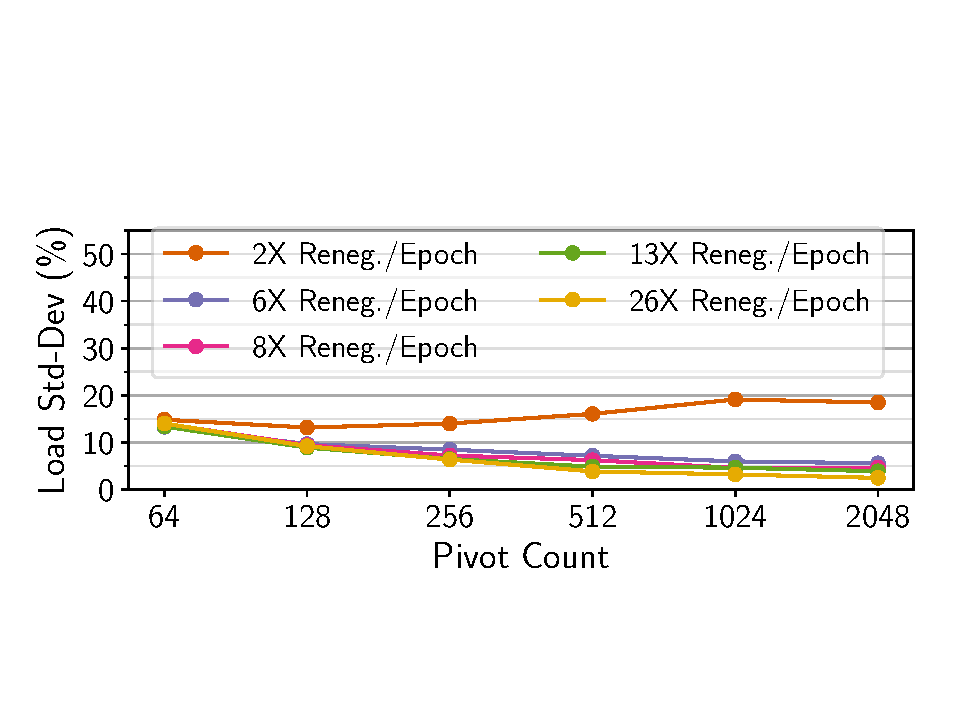
\includegraphics[trim=0.6cm 2.5cm 0.6cm 3.6cm,clip,width=\columnwidth]{data/figs/carp_load.vs.params.pdf}
  \caption{Impact of CARP parameters on partition load balance}
  \label{fig:carp:eval-rtpload}
}

\newcommand{\figevalrtprt}{
  \centering
  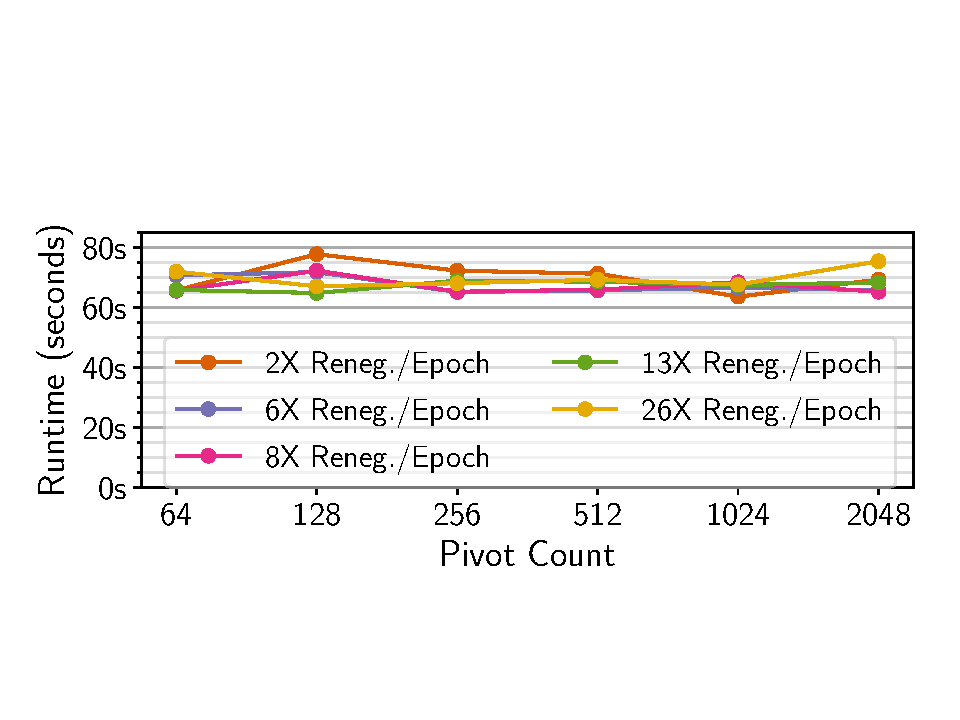
\includegraphics[trim=0.6cm 2.5cm 0.6cm 3.6cm,clip,width=\columnwidth]{data/figs/carp_runtime.vs.params.pdf}
  \caption{Impact of CARP parameters on write performance}
  \label{fig:carp:eval-rtprt}
}
